\documentclass{overturerep}
\usepackage{url}
\usepackage{graphics}
\usepackage{times}
\usepackage{listings}
\usepackage{color}
\usepackage{graphicx}
\usepackage{latexsym}
\usepackage{longtable} % ,multirow}

\newcommand{\vdmtools}{VDMTools}
\newcommand{\vdmstyle}[1]{\texttt{#1}}
\newcounter{exerciseno}

%\newcommand{\Exercise}[1]{%
%    \textbf{Exercise \thechapter.\theexerciseno}
%   \refstepcounter{exerciseno} #1 $\Box$\\ }%}
%\newcommand{\initexercise}{\setcounter{exerciseno}{0}}
%\newcounter{exerciseno}

\newcommand\thebookexercise{\thechapter.\arabic{exerciseno}}
\newenvironment{myexercise}{\par
  \refstepcounter{exerciseno}%
  \indent\textbf{Exercise\ \thebookexercise}\enskip}{$\Box$\\
}
\newenvironment{myhardexercise}{\par
  \refstepcounter{exerciseno}%
  \indent\textbf{Exercise\ \thebookexercise $\star$}\enskip}{$\Box$\\
}
\newcommand{\initexercise}{\setcounter{exerciseno}{0}}
\newenvironment{mysolution}{
} %% This will be replaced by a perl script extracting the solutions
  %% and inserting them automatically into the solutions chapter.
 
%\newcommand{\insertcommentedvdm*}[2]{}
  %% This macro is identified by perl script which will move the
  %% parameter to the solutions chapter.
% definition of VDM++, JavaCC, JJTree, JTB, ANTLR and SableCC for listings
\lstdefinelanguage{VDM++}
  {morekeywords={act, active, fin, req, waiting, abs, all, allsuper, always, and, answer, 
     assumption, async, atomic, be, bool, by, card, cases, char, class, comp, compose, conc, cycles,
     dcl, def, definitions, del, dinter, div, dlmodule, do, dom, dunion, duration, effect, elems, else, elseif, end,
     error, errs, exists, exists1, exit, exports, ext, floor, for, forall, from, functions, 
     general, hd, if, imports, in, inds, infer, init, inmap, input, instance, int, inter, inv, inverse, iota, is, 
     isofbaseclass, isofclass, inv, inverse, lambda, len, let, map, measure, mu,
     mutex, mod, module, nat, nat1, new, merge, 
     munion, not, of, operations, or, others, per, periodic, post, power, pre, pref, 
     private, protected, public, qsync, rd, responsibility, return, reverse,  
     sameclass, parameters, psubset, rem, renamed, rng, sel, self, seq, seq1, set, skip, specified, st, 
     start, startlist, state, static, subclass, subset, subtrace, sync, system, then, thread, 
     threadid, time, tixe, tl, to, token, traces, trap, types, undefined,
     union, uselib, using, values, 
     variables, while, with, wr, yet, RESULT, false, true, nil, periodic pref, rat, real},
   %keywordsprefix=mk\_,
   %keywordsprefix=a\_,
   %keywordsprefix=t\_,
   %keywordsprefix=w\_,
   sensitive,
   morecomment=[l]--,
   morestring=[b]",
   morestring=[b]',
  }[keywords,comments,strings]
\lstdefinelanguage{JavaCC}
  {morekeywords={options, PARSER\_BEGIN, PARSER\_END, SKIP, TOKEN},
   sensitive=false,
  }[keywords]

% define the layout for listings
\lstdefinestyle{tool}{basicstyle=\ttfamily,
                         frame=trBL, 
			 showstringspaces=false, 
			 frameround=ffff, 
			 framexleftmargin=0mm, 
			 framexrightmargin=0mm}
\lstdefinestyle{mystyle}{basicstyle=\ttfamily,
                         frame=trBL, 
%                         numbers=left, 
%			 gobble=0, 
			 showstringspaces=false, 
%			 linewidth=\textwidth, 
			 frameround=fttt, 
			 aboveskip=5mm,
			 belowskip=5mm,
			 framexleftmargin=0mm, 
			 framexrightmargin=0mm}
%\lstdefinestyle{mystyle}{basicstyle=\sffamily\small,
%			 frame=tb,
%                         numbers=left,
%			 gobble=0,
%			 showstringspaces=false,
%			 linewidth=345pt,
%			 frameround=ffff,
%			 framexleftmargin=8mm,
%			 framexrightmargin=8mm,
%			 framextopmargin=1mm,
%			 framexbottommargin=1mm,
%			 aboveskip=7mm,
%			 belowskip=5mm,
%			 xleftmargin=10mm,}

\lstset{style=mystyle}
\lstset{language=VDM++}
\lstset{alsolanguage=Java}
% The command below enables you to escape into normal LaTeX mode inside your 
% VDM chunks by starting with a `?� character and ending with a `��
\lstset{escapeinside=?�}

\newcommand{\kw}[1]{{\tt #1}}

%%%%%%%%%%%%%%%%%% Commands for bibtex %%%%%%%%%%%%%%%%%%%%%%%
%************************************************************************
%                                                                       *
%       Bibliography and Terminology supporting commands                *
%                                                                       *
%************************************************************************

\newcommand{\bthisbibliography}[1]{\chapter*{References}%
   \begin {list} {}%
     {\settowidth {\labelwidth} {[#1]XX}%
      \setlength {\leftmargin} {\labelwidth}%
      \addtolength{\leftmargin} {\labelsep}%
      \setlength {\parsep} {1ex}%
      \setlength {\itemsep} {2ex}%
     }
  }
\newcommand{\ethisbibliography}{\end{list}}
\newcommand{\refitem}[2]
  {\bibitem[#1]{#2}}

% Requirements environment
\newenvironment{reqs}{%
\begin{enumerate}
%\renewcommand{\labelenumi}{\textbf{R\theenumi}}
\renewcommand{\theenumi}{\textbf{R\arabic{enumi}}}
}{%
\end{enumerate}}

%\newcommand{\Exercise}[1]{%
%    \textbf{Exercise \thechapter.\theexerciseno}
%   \refstepcounter{exerciseno} #1 $\Box$\\ }%}
%\newcommand{\initexercise}{\setcounter{exerciseno}{0}}

\newcommand{\experience}[1]{%
\begin{center}
\fbox{
\begin{minipage}[t]{.8\textwidth}
#1
\end{minipage}}
\end{center}}

\usepackage{fancyhdr}

\pagestyle{fancy}
\fancyhead{}
\fancyhead[LO]{\leftmark}
\fancyhead[RE]{Tutorial to Overture/VDM-RT}
\fancyhead[RO,LE]{\resizebox{0.05\textwidth}{!}{
\includegraphics{OMLlogoattempt.jpg}}}
\fancyfoot[C]{\thepage}

\begin{document}
 
\title{Tutorial to Overture/VDM++}
\author{Peter Gorm Larsen\\
        %\and
        John Fitzgerald \\
        %\and
        Sune Wolff\\
        %\and
        Nick Battle\\
        Kenneth Lausdahl\\
        Augusto Ribeiro\\
        Kenneth Pierce}

\date{January 2010}

%\frontmatter
\reportno{TR-2010-01}     

\pagenumbering{roman}
\maketitle
%\addtocounter{page}{2}
\tableofcontents
\newpage
% \include{foreword/foreword}

%\cleardoublepage
%\mainmatter
%\lhead{\nouppercase{\rightmark}}
%\rhead{\nouppercase{\leftmark}}


%\pagestyle{fancy}
%\fancyhead{}
%\fancyhead[LO]{\leftmark}
%\fancyhead[RE]{Validated Designs for Object-oriented Systems}
%\fancyhead[RO,LE]{\thepage}
%\fancyfoot{}
%%\fancyfoot[LE,RO]{\thepage}

\pagenumbering{arabic} 
\setcounter{page}{1}
\addtocounter{chapter}{2}

% $Revision: 1.28 $
\chapter{Overture Tool Support for VDM++: an Introductory Guide}\label{cha:toolbox}
% vppinput[guide/test1.vpp]
\initexercise

% \section*{Aims}
\section*{Preamble}

This is an introduction to the Overture Integrated Development
Environment (IDE) and its facilities for supporting modelling and
analysis in VDM++. It may be used as a substitute for Chapter 3 of
``Validated Designs for Object-oriented Systems''\footnote{John
  Fitzgerald, Peter Gorm Larsen, Paul Mukherjee, Nico Plat and Marcel
  Verhoef. \emph{Validated Designs for Object-oriented Systems},
  Springer, New York. 2005, ISBN 1-85233-881-4} or as a free-standing
guide. Additional material is available on the book's web
site\footnote{\url{www.vdmbook.com}.}. Throughout this guide we will refer to
the textbook as ``the book'' and the book's web site simply as ``the
web site''.

We use examples based on the \emph{alarm} case study introduced in
Chapter~2 of the book. For readers using this as a
free-standing guide, an informal explanation of the case study and its
VDM++ model are given in Appendix~\ref{app:alarm}. The model has been slightly
extended from the original version in order to illustrate Overture's
test automation features.

We introduce the features of Overture that support the combination of
formal modelling in VDM++ with object-oriented design using UML. This
is done by providing a ``hands-on'' tour of Overture, providing enough
detail to allow you to use Overture for serious applications,
including the exercises in the book. However, this is by no means a
complete guide to Overture; more information can be obtained
from~\url{www.overturetool.org}.


% Full details are provided in the user manuals accessible via the book's Web
% site (\bookurlshort).



\section{Introduction}

One of the main benefits of combining VDM++ and UML class diagrams and
sequence diagrams is
the ability to use software tools to assist in the analysis of the
models. Often the analytic power of UML models alone can be limited as
many tools concentrate on just the structural view of
classes. However, the combination of Enterprise Architect (EA) and
Overture provides a significant number of benefits.

This guide can be used to illustrate the combination of Enterprise
Architect and
Overture support, or just Overture support if EA is
not available or desired.

Section~\ref{sec:install} describes how to obtain the tools and the
license for EA. For those readers who would like to start using
EA, Section~\ref{sec:Rose} briefly explains how a
first model can be built in UML.  Section~\ref{sec:vdmsupport}
provides an initial introduction to the terminology used by Eclipse
tools like Overture. Section~\ref{sec:fromUMLtoVDM} shows how to
import EA UML class and sequence diagrams into Overture and
export them back to UML again. The round-trip engineering abilities of
this link however is still at a prototype stage so if you wish to use
this you have to expect that this part is still not as automatic as we
would like. 
% This includes how to use Overture to configure a VDM++ project, perform static
% checking and synchronise definitions for all classes with an Enterprise
% Architect model, if desired.
Section~\ref{sec:debugging} describes the process of testing and
debugging using Overture. Section~\ref{sec:testcov}  describes how
line coverage from using the debugger can be covered and displayed. 
Section~\ref{sec:CT} shows how parts of the test process can be 
automated using Overture's combinatorial testing feature.  
Section~\ref{sec:PO} demonstrates how it is possible automatically 
to generate the additional checks (called \emph{proof obligations}) needed ensure that a model is
consistent.  Finally, Section~\ref{sec:cmdline} illustrates how parts
of Overture's functionality can be accessed from a command line.

%including support for test coverage analysis which is not currently
%available from the Eclipse GUI.
% internal consistency checking facilities can be used to identify potential
% sources of run-time errors. Finally the section provides a brief introduction
% to further functionality from Overture used later in this book. The tables
% illustrating the different kinds of buttons from Overture all contain a column
% called ``Used'' indicating whether the use of the corresponding button is
% covered by this chapter.



\section{Obtaining the Tools}\label{sec:install}

In order to run the examples and exercises presented in the book, it
is necessary to install two separate tools -- Overture and Enterprise
Architect, the latter being license-controlled. 
\begin{description}
%\item[VDM++ Lite:] This is an educational version of the VDM++ Toolbox
%from IFAD A/S which can be used purely for academic purposes. This
%tool has an upper limit on the size of models which can be
%handled. However, it can be used with all the examples from this book.
\item[\textbf{Overture:}] This is an open source tool developed by a
  community of volunteers and built on the Eclipse platform. The
  Overture development project is managed on
  SourceForge\footnote{\url{https://sourceforge.net/projects/overture/}}.
%There are two ways of obtaining the Overture Eclipse plug-in. 
%If
%you are already a user of Eclipse (version 3.5 or later) you can install the
%plug-in from an update site:
%  \begin{quote}
%  (\texttt{http://www.overturetool.org/updatesite/}). 
%  \end{quote}
The best way to run Overture is to download a special version of
  Eclipse with the Overture functionality already
  pre-installed. If you go to
  \begin{quote}
  \url{http://sourceforge.net/projects/overture/files/}
  \end{quote}
  \noindent you can find pre-installed versions of Overture for
  Windows, Linux and Mac\footnote{It is planned to develop an update facility,
  allowing updates to be applied directly from within the generic
  Eclipse platform without requiring a reinstallation. However, this can be a
  risky process because of the dependencies on non-Overture components
  and so is not yet supported.}.

\item[\textbf{Enterprise Architect:}] This is a commercial tool from a
  company called SparxSystems. The product, and a free evaluation license, can be
  obtained from 
\begin{quote}
\texttt{http://www.sparxsystems\-.com\-.au/}.
\end{quote}

%\item[\textbf{Rational Rose}$^{\mbox{\small\textbf{{\textregistered}}}}$:]
%\sindex{Rational Rose@\tool{Rational
%Rose$^{\mbox{\small\textbf{{\textregistered}}}}$}|textbf} This is the
%commercial version of Rational
%Rose from Rational, now
%owned by IBM. It is necessary to either purchase a license for this
%tool or get a free evaluation license. This tool is under continually
%being improved so again you should visit the book's Web
%site~(\bookurlshort) for instructions on how to obtain the most recent
%installation. In the rest of this book we will simply use the term
%``Rose'' to refer to this tool.
\end{description}

A large library of sample VDM++ models, including all those needed
for the exercises in the book, is available and can be downloaded from
SourceForge under the \texttt{examplesPP.zip} file using the
URL\footnote{The library files are created to be used with Eclipse,
  but can be opened with file compression programs like \texttt{Winrar} on
  Windows.}:
\begin{quote}
\url{https://sf.net/projects/overture/files/Examples/}
\end{quote}
You can import the example library zip folder as described in
Section~\ref{sec:vdmsupport}.  Finally, the web site
\texttt{www.vdmbook.com} contains all the examples used in this book
as plain text files but these are also all present in the above
mentioned zip file. Finally, in order to make use of the
test coverage feature described in Section~\ref{sec:testcov} it is
necessary to have the text processing system called \LaTeX\ and its
\texttt{pdflatex} feature. This can for example be obtained from:
\begin{quote}
\url{http://miktex.org/2.8/}
\end{quote}


\paragraph{Note for \vdmtools$^{\mbox{\small\textbf{{\textregistered}}}}$ users.} 
Overture provides a new open source VDM tool set, but it can
also work with
\vdmtools$^{\mbox{\small\textbf{{\textregistered}}}}$. \vdmtools, originally developed IFAD A/S, is now
maintained and developed by CSK Systems~(see
\url{http://www.vdmtools.jp/en/}). In the future Overture will be able
to accesses
\vdmtools\ functionality via a remote API, but the integration will to
some extent be limited by the API capabilities. However, the additional
features of the Overture IDE make it worth considering as a front end
to the \vdmtools\ functionality.

% Distribution and licensing arrangements change with time, so you should visit
% the book's Web site~(\bookurlshort) for instructions on how to obtain the most
% recent installation and getting any associated manuals.

% Overture has a feature for automatically converting VDM++ models back and forth
% to UML for Enterprise Architect using a file based interface called XMI.

 
\section{Using Enterprise Architect}\label{sec:Rose}

This section describes the tool support available if you wish to start
model construction using UML class diagrams. 

The \texttt{alarmumlinit.eap} file can be found on the book's web
site. This UML class diagram model is identical to the initial class
diagram from the previous chapter 
except that the \vdmstyle{Plant} class has been updated with the three
operations identified in Appendix~\ref{app:alarm}.
% chapter~2. 
Note that the operations have not yet been given signatures. Download
this \texttt{.eap} file and open it using Enterprise Architect. When
this model is open, the class diagram should look like that shown in 
Figure~\ref{fig:initialuml}.

\begin{figure}[htbp]
\begin{center}
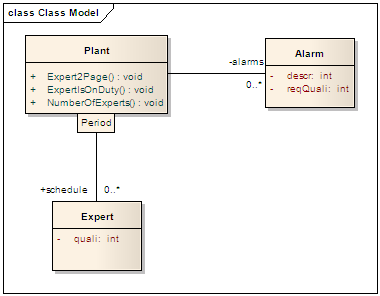
\includegraphics[width=4in]{figures/initialumloverture}
\caption{The initial UML class diagram.\label{fig:initialuml}}
\end{center}
\end{figure}

The small `\texttt{+}' next to the r\^{o}le name \texttt{schedule}
indicates that this association is \kw{public}. The `\texttt{-}' in
front of the r\^{o}le name \texttt{alarms} indicates that it is
\kw{private}. You can change the visibility of the
\texttt{schedule} association to \kw{private} by double-clicking the
association and changing the \textsf{Association properties} with the
\textsf{target Role}, changing the \textsf{Access} field.

You can update the signatures for the operations in the
\vdmstyle{Plant} class. However, this is awkward and most developers
prefer to use a text editor to perform such updates in the VDM++ text, then converting back to the 
UML model automatically.

To convert a UML class diagram model to a VDM++ model, you first need
to export the UML model from EA to XMI format~(see Figure~\ref{fig:xmiexport}). This
is then subsequently imported into Overture as will be explained in Section~\ref{sec:fromUMLtoVDM}.

\begin{figure}[htbp]
\begin{center}
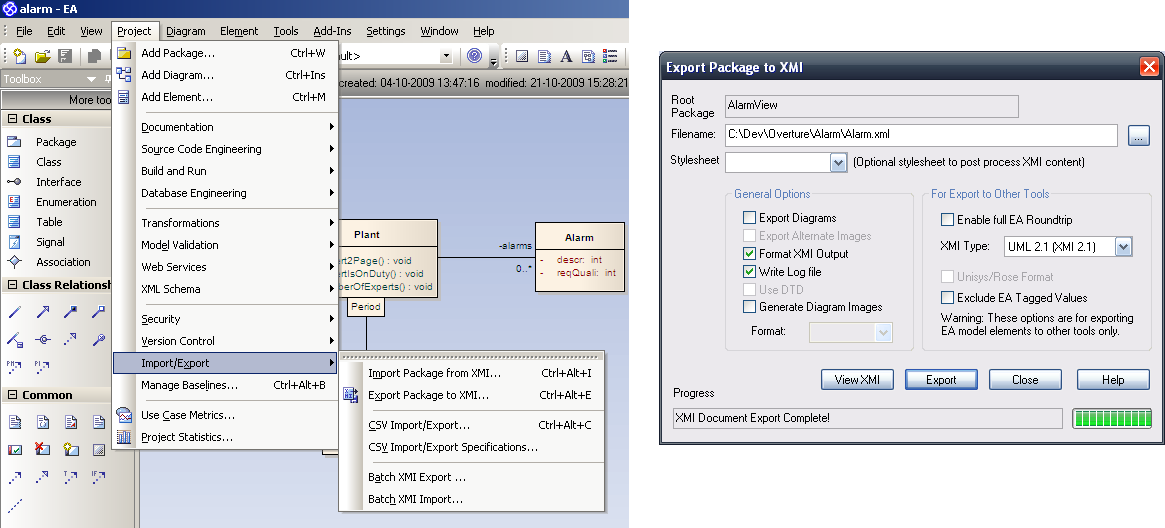
\includegraphics[width=4.5in]{figures/xmiexport}
\caption{Exporting the UML model to XMI format.\label{fig:xmiexport}}
\end{center}
\end{figure}

%The graphical user interface for Overture partly uses buttons, menus and
%automatic checking to invoke the major functionality.

% As each area of the tools' functionality is introduced, a table gives the icons
% on the relevant buttons. It is also indicated whether the buttons are directly
% referred to in this chapter.
 
% \begin{table} \begin{center} \caption{\vdmtools\ project
% buttons\label{tab:project}} \begin{tabular}{|l|c|l|}\hline \hline
% \textbf{Button} & \textbf{Used} & \textbf{Explanation} \\ \hline
%\includegraphics[width=0.06\textwidth]{projectnew} & No & Create a new project \\
%\includegraphics[width=0.06\textwidth]{load} & No  & Load an existing project \\
%\includegraphics[width=0.06\textwidth]{projectsave} & Yes & Save the current project \\
%\includegraphics[width=0.06\textwidth]{projectsaveas} & No & Save the current project under a new name \\
%\includegraphics[width=0.06\textwidth]{plus} & Yes & Add selected files to project \\
%\includegraphics[width=0.06\textwidth]{minus}& Yes & Remove selected files from project \\
%\includegraphics[width=0.06\textwidth]{projectoptions} & Yes & Show and edit current project options \\
%\includegraphics[width=0.06\textwidth]{tooloptionsbutton} & Yes & Select tool options \\
% \hline \hline \end{tabular} \end{center} \end{table}


\section{Using the Overture Perspective}\label{sec:vdmsupport}

Eclipse is an open source platform based on a \emph{workbench} that
provides a common look and feel to a large collection of extension
products. Thus if a user is familiar with one Eclipse product, it will
generally be easy to start using a different product on the same
workbench. The Eclipse workbench consists of several panels known as
\emph{views}, such as the Script Explorer view at the top left of
Figure~\ref{fig:OverturePerspective}. A particular
collection of panels designed to assist a specific activity is called
a \emph{perspective}. For example
Figure~\ref{fig:OverturePerspective} shows the standard
Overture perspective which contains views for managing Overture
projects, viewing and editing files. As we shall see later, several
other perspectives are also available in Overture.

\begin{figure}[!htb]
\begin{center}
  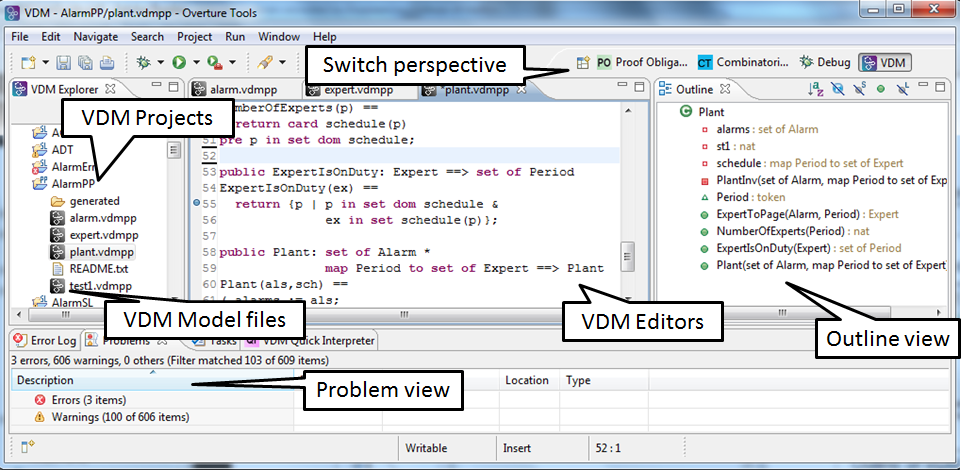
\includegraphics[width=5in]{figures/OverturePerspective}
  \caption[labelInTOC]{The Overture Perspective}
  \label{fig:OverturePerspective}
\end{center}
\end{figure}

The \emph{Script Explorer view} allows you to create, select, and
delete Overture projects and navigate between the files in these
projects. Start by importing the alarm project from zip file mentioned
above. This can be done by right clicking the project view
and selecting \emph{Import}, followed by \emph{General} $\rightarrow$
\emph{Existing Projects into Workspace}.  In this way the projects
from \texttt{.zip} file mentioned above can be imported easily. Initially it is
recommended that you only import the \texttt{AlarmErrPP} and the
\texttt{Alarm++tracesPP} projects as shown in
Figure~\ref{fig:importalarm}\footnote{You need both of these for
  carrying out different kinds of exercises throughout this chapter.}.

\begin{figure}[!htb]
\begin{center}
  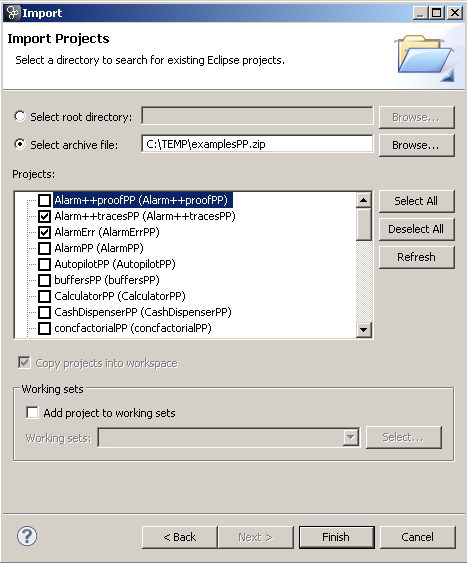
\includegraphics[width=2.5in]{figures/importalarmprofs}
  \caption[labelInTOC]{Importing the \texttt{Alarm} VDM++ Projects}
  \label{fig:importalarm}
\end{center}
\end{figure}

An editor customised to the dialect of VDM being used in the project
will appear when one of the imported files are selected in the
Explorer view by double clicking. When the
\texttt{AlarmErrPP} project has been imported one can right click on the
project in the \emph{Explorer} view and then select the
\texttt{Properties} item in the menu and then
Figure~\ref{fig:settings} will pop up. This includes the properties set
for this project including specific VDM options. Note that there is a 
language version option that for the \texttt{AlarmErrPP}
project set to \texttt{vdm10} which indicates that it include
non-standard features such as {\bf\ttfamily traces} which is explained 
in Section~\ref{sec:CT}. In addition, options are gathered here for 
additional checks where the \texttt{AlarmErrPP} project simply follow 
the standard settings used for new projects.

\begin{figure}[!htb]
\begin{center}
  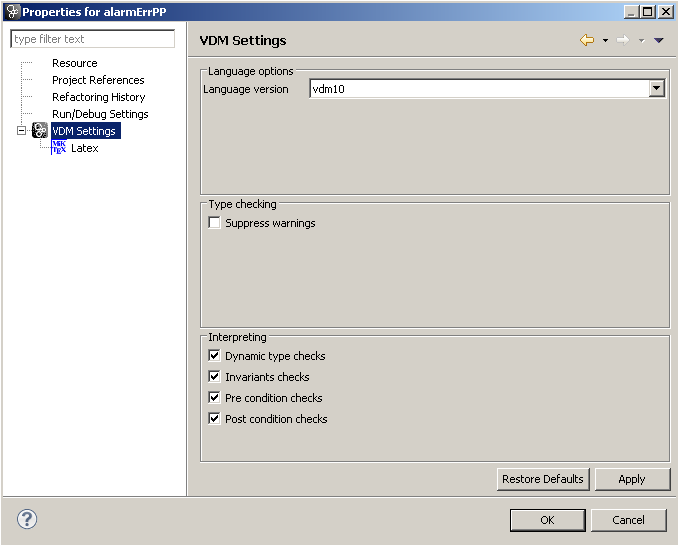
\includegraphics[width=4.0in]{figures/settings}
  \caption[labelInTOC]{Properties for the \texttt{AlarmErrPP} Project}
  \label{fig:settings}
\end{center}
\end{figure}

%A new VDM++ project is created by choosing
%\emph{File} $ \rightarrow$ \emph{New} $\rightarrow$
%\emph{Project}. The dialog shown in
%Figure~\ref{fig:newOvertureProjectPP} will appear. Click \emph{Next}
%and name the project.

%\begin{figure}[!htb]
%\begin{center}
%  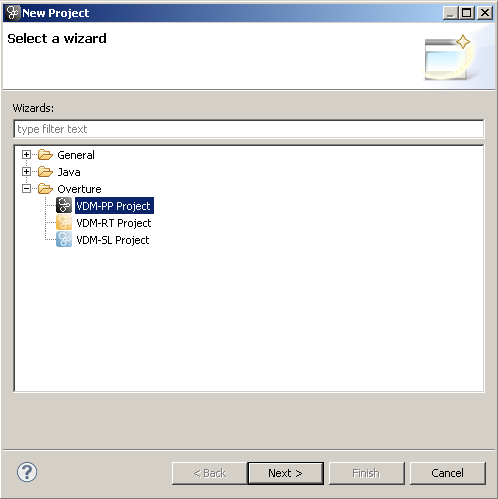
\includegraphics[width=2.5in]{figures/newoverturePPproject}
%  \caption[labelInTOC]{Creating a New VDM++ Project}
%  \label{fig:newOvertureProjectPP}
%\end{center}
%\end{figure}

The \emph{Outline view}, to the right of the editor (see
Figure~\ref{fig:OutlineView}) displays an outline of the file selected
in the editor. It shows all declared classes, their instance variables,
values, types, functions, operations and traces.
Figure~\ref{fig:OverturePerspective} shows the outline view on the
right hand side. Clicking on an operation or function will move the
cursor in the editor to the definition of that operation/function. At
the top of the outline view there is a button to (optionally) order
the elements of the outline view alphabetically.

\begin{figure}[!htb]
\begin{center}
  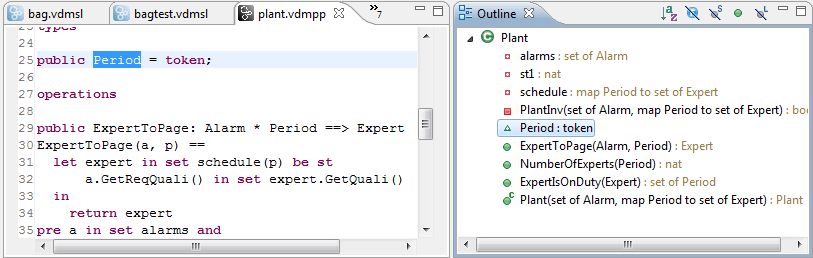
\includegraphics[width=4.5in]{figures/OutlineView}
  \caption[labelInTOC]{The Outline View}
  \label{fig:OutlineView}
\end{center}
\end{figure}

The \emph{Problems view} presents information about all the open projects you
are working on, such as warning and error messages. In
Figure~\ref{fig:OverturePerspective} the problems view is shown at the bottom.

Most of the other features of the workbench, such as the menus and
toolbars, are similar to those used in other Eclipse applications,
though it is worth noting that there is a special menu with
Overture-specific functionality. One convenient feature is a toolbar
that appears on the right side of the screen and allows the user to
switch between perspectives; the particular perspectives on show here
vary dynamically according to history.

\section{Getting Started using Templates}\label{sec:templates}

Before proceeding, please make sure that you have imported both the
\texttt{AlarmErrPP} and the \texttt{Alarm++tracesPP} projects as shown in
Figure~\ref{fig:importalarm}. When editing a VDM++ model, the Overture IDE parses the content of the
editor buffer continuously as changes are made. Any parse errors will
be reported in the problems view, as well as being highlighted in the
editor. See the bottom of Figure
\ref{fig:OverturePerspective}. Each time a VDM++ model file is
saved the editor type-checks the model and reports any errors or
warnings. Note also that the suggestions made in the error messages
may not always be entirely the action you may wish to take when
correcting the source since the tool cannot guess what you intended
to write.

Templates can be particularly useful when modifying VDM++ models. If you hit
the key combination \textit{CTRL+space} after the initial characters
of the template needed, Overture triggers a proposal. For example, if
you type ''op'' followed by \textit{CTRL+space}, the Overture IDE
will propose the use of an implicit or explicit operation template as
shown in Figure~\ref{fig:operationTemplate}. The Overture IDE
supports several types of template: cases, quantifications, functions
(explicit/implicit), operations (explicit/implicit) and many
more. Additional templates can easily be added in the future. The use
of templates makes it much easier for users lacking deep familiarity
with VDM syntax to nevertheless construct models.

\begin{figure}
	\begin{center}
	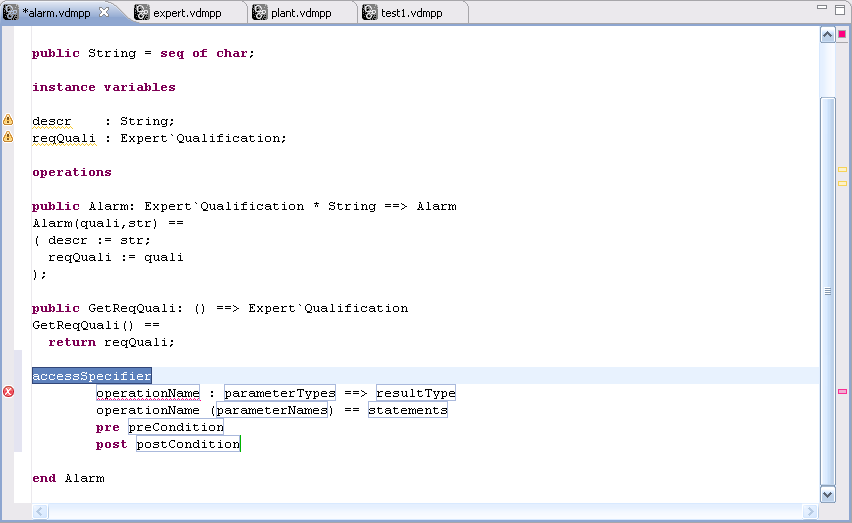
\includegraphics[width=4in]{figures/OperationTemplate}
	\caption{Explicit operation template}
	\label{fig:operationTemplate}
	\end{center}
\end{figure}

A new VDM++ project is created by choosing \emph{File} $ \rightarrow$
\emph{New} $\rightarrow$ \emph{Project}. The dialog box shown in
Figure~\ref{fig:newoverturePPproject} will appear. Ensure that VDM++
is selected as the project type, click \emph{Next} and then name the
project \texttt{Test} and if next is selected again it gets possible
to select standard libraries as shown in
Figure~\ref{fig:stdlibs}. These standard libraries require users to
make use of modules but in return it is possible to get standard
input/output, math and general utility functionality by selecting the
appropriate standard libraries. In this \texttt{Test} project we can
try to select the \texttt{IO} standard library. Afterwards one simply
select \texttt{Finish}. Now you have an almost empty project (with the
exception of the \texttt{IO.vdmpp} file in the \texttt{lib} directory)
and you can then either add new VDM++ files to the project or simply paste in existing
VDM++ source files from elsewhere. Adding a VDM++ file to a project
you can rightclick on the project and then select \emph{New}
$\rightarrow$ \emph{VDM++ Class} and then give a meaning full name
(e.g.\ \texttt{Test}) to the class you would like to start defining and press
\texttt{Finish}. This will create a new class file with the
selected name and with space for the different kinds of definitions
you can make inside such a VDM++ class.

\begin{figure}[!htb]
\begin{center}
  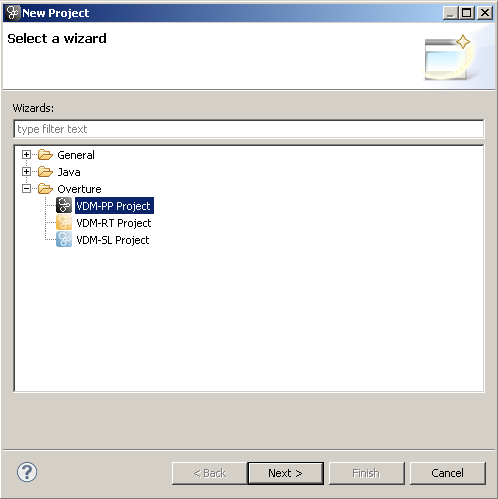
\includegraphics[width=2.5in]{figures/newoverturePPproject}
  \caption[labelInTOC]{Creating a New VDM++ Project}
  \label{fig:newoverturePPproject}
\end{center}
\end{figure}

\begin{figure}[!htb]
\begin{center}
  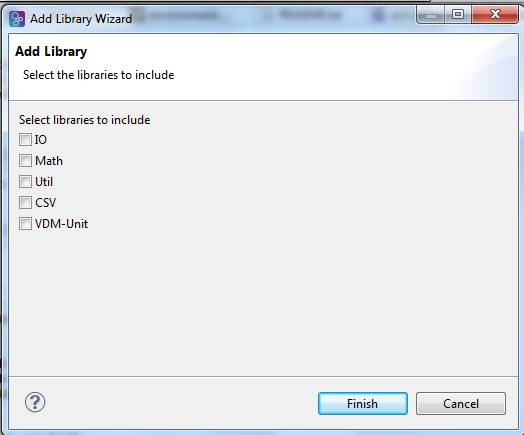
\includegraphics[width=2.5in]{figures/stdlibs}
  \caption[labelInTOC]{The VDM++ Standard Libraries}
  \label{fig:stdlibs}
\end{center}
\end{figure}

\section{Mapping UML to  VDM}\label{sec:fromUMLtoVDM}\label{sec:syntaxcheck}
\label{sec:typecheck}

In order to map the UML class diagram created in Enterprise Architect
to VDM, a new project must be created in the Overture tool to receive
it. This is done by right-clicking in the \emph{Script Explorer} view,
and creating a new VDM-PP project and for example naming it
\texttt{AlarmUML}. By right-clicking the new project
root in the \emph{Script Explorer}, \emph{UML Transformation} can be
chosen, followed by \emph{Import XMI}. Now browse to the XMI/XML file
exported from EA and open this.

The three classes from the Alarm system will be converted to VDM++ format
(\texttt{.vdmpp}), one file per class.

%When editing a model, it can be useful to navigate to a specific
%operation in the file, instead of reaching for the mouse, this can be
%done using a shortcut (\textit{Ctrl+O})) which opens a small pop-up. This
%pop-up allows the user to navigate to a given location in the model
%simply by filling out the name of an field, operation, function or
%type. The use of intellisense furthermore ensures that the user does
%not have to write out the full name of the desired location. Figure
%\ref{fig:quickOutline} shows the quick outline.

%\begin{figure}
%	\begin{center}
%	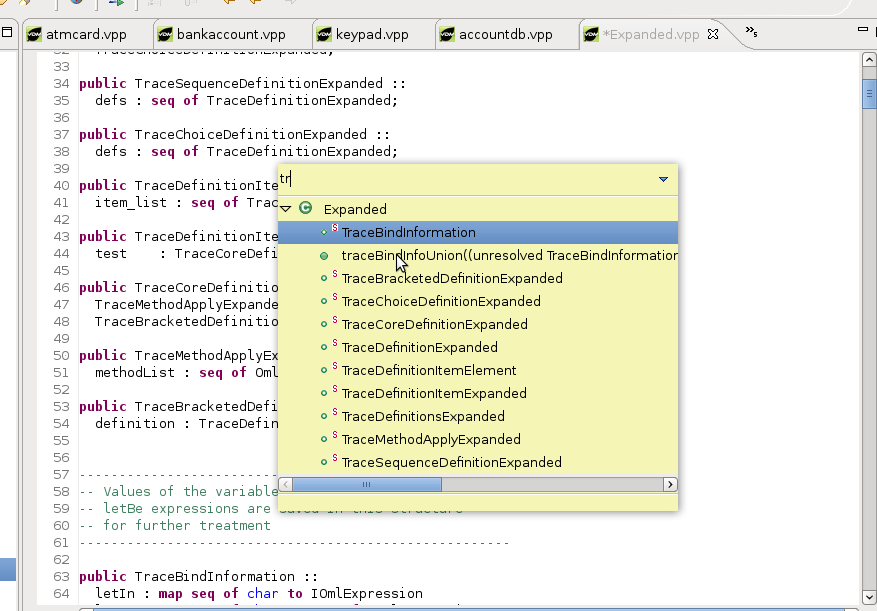
\includegraphics[width=300px]{figures/quickOutline}
%	\caption[Quick Outline]{Quick Outline}
%	\label{fig:quickOutline}
%	\end{center}
%\end{figure}

The transformation from UML to VDM is not entirely automated in the
current release. For
example, any custom types are transformed to VDM++ definitions using
machine-generated identifiers since custom types are not named in
UML. As a result, you have to expect to make minor modifications to
the generated VDM files. 

%When making corrections to the model, you can
%use the Overture IDE templates. When you hit the key combination
%\textit{CTRL+space} after entering the initial characters of the
%template needed, Overture will offer possible completions. For
%example, if you type ''op'' followed by \textit{CTRL+space}, Overture
%will propose the use of an implicit or explicit operation template. An
%example of this can be seen in Figure~\ref{fig:operationTemplate}.
%
%\begin{figure}
%	\begin{center}
%	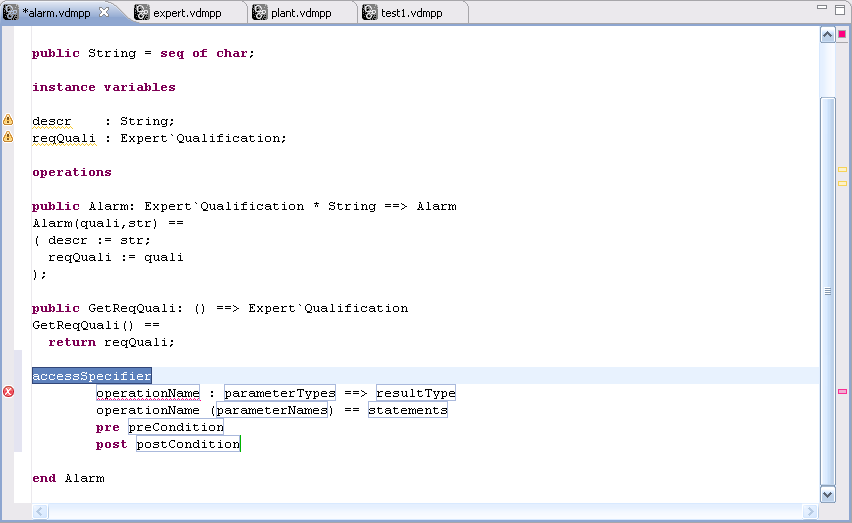
\includegraphics[width=4in]{figures/OperationTemplate}
%	\caption{Explicit operation template}
%	\label{fig:operationTemplate}
%	\end{center}
%\end{figure}

%The Overture IDE supports many templates for language constructs
%including cases statements, classes, quantified expressions, functions
%(explicit/implicit), operations (explicit/implicit) and many
%more. Further templates can easily be added in the future. The use of
%templates makes it more concenient to write VDM models without
%detailed prior knowledge of the language syntax.

Before proceeding, finish the model of the alarm system. Begin by
deleting the alarm project in the Overture IDE, and import the alarm
project from the book's web site. This can be done by right clicking
the project view and selecting \emph{Import}, followed by
\emph{Existing Projects into Workspace}.

When editing a VDM model, the Overture IDE parses the content of the
editor buffer continuously as changes are made. Any parsing errors
will be reported in the problems view, as well as being highlighted in
the editor~(see the bottom of
Figure~\ref{fig:OverturePerspective}). Each time a VDM model is saved
the editor type checks the entire VDM++ model and reports any errors or
warnings. Note also that the suggestions about missing characters 
made in the error messages
may not always be entirely the action you may wish to take when
correcting the source since the tool cannot guess what you intended to
write.

The imported \texttt{AlarmErrPP} project contains a number of VDM++
model files with a number of
deliberate errors.  The errors are common ones such a
semicolons separating definitions that has been forgotten.

\begin{myhardexercise}\label{ex:type-errors}
Correct all the errors discovered by the syntax and type checker from
Overture and save the corrected files. Continue this process until no errors appear.
\textbf{Hint:} Consult the model presented in 
Appendix~\ref{app:alarm}
%Chapter~\ref{cha:guide} 
to see how values (note using ``\vdmstyle{=}'' rather than
``\vdmstyle{:=}''), types and constructors should be defined and how
access modifiers should be used.
\end{myhardexercise}


\subsection{Mapping VDM to UML}

After correcting all the errors in the \texttt{AlarmErrPP} project, it is possible
to map the complete VDM model to UML. To do this, simply right
click the project root and choose \emph{UML Transformation} $
\rightarrow $ \emph{Export XMI}. The XMI file can subsequently be
imported in EA, enabling the user to get an overview
of the complete model.

\begin{myexercise}\label{ex:rosemapping}
Add an instance variable to one of the other classes at the VDM++
level. Save it and it will automatically be syntax and type checked at
the VDM++ level. Then export the model to XMI in order to see your
changes in EA.
\end{myexercise}



\section{Debugging}\label{sec:debugging}

This section describes how to debug a model by testing it using the
Overture IDE. The following test file (\texttt{Test1.vdmpp}) can be
found in the alarm project and it is provided in
Appendix~\ref{sec:VDMModel}.

\lstset{language=VDM++}
%\begin{lstlisting}
class Test1

instance variables

a1   : Alarm  := new Alarm(<Mech>,"Mechanical fault");
a2   : Alarm  := new Alarm(<Chem>,"Tank overflow");
ex1  : Expert := new Expert({<Mech>,<Bio>});
ex2  : Expert := new Expert({<Elec>});
ex3  : Expert := new Expert({<Chem>,<Bio>,<Mech>});
ex4  : Expert := new Expert({<Elec>,<Chem>});
plant: Plant  := new Plant({a1},{p1 |-> {ex1,ex4},
                                 p2 |-> {ex2,ex3}});

values

p1: Plant`Period = mk_token("Monday day");
p2: Plant`Period = mk_token("Monday night");
p3: Plant`Period = mk_token("Tuesday day");
p4: Plant`Period = mk_token("Tuesday night");

operations

public Run: () ==> set of Plant`Period * Expert
Run() == 
  let periods = plant.ExpertIsOnDuty(ex1),
      expert  = plant.ExpertToPage(a1,p1)
  in 
    return mk_(periods,expert);

end Test1
\end{lstlisting}



Using this test, it is possible to exercise the system informally in
order to check if the correct expert is paged as a result of a given
alarm.


\subsection{The Debug Configuration}

Before the debugging can begin in Overture, a debug configuration must
be created by right clicking the project and choosing \emph{Debug As}
$ \rightarrow $ \emph{Debug configuration}\footnote{Note that the
  \emph{Run As} functionality existing Eclipse users are used to is
  not supported in the current version of Overture.}. The debug configuration
dialog requires the project name and the class and the operation/function
used as the entry point of the test.  Figure~\ref{fig:debugConfiguration}
shows the debug configuration for the alarm model. The class and
operation/function name can be chosen from a Browse dialog; if the
operation or function has arguments, these must be typed in manually
between the brackets of the entry point
function/operation\footnote{Note that in the current version of
  Overture the error handling is not optimal if you type something
  that is not defined here. If you make mistakes here the current
  version will normally come with an error message like ``Execution
  error 206: Unexpected token in expression'' in the \emph{Console} view}.

\begin{figure}[htp]
\begin{center}
  \includegraphics[width=4in]{figures/DebugConfiguration}
  \caption{The debug configuration dialog}
  \label{fig:debugConfiguration}
\end{center}
\end{figure}

Once the debug configuration is ready, the model can be debugged. This
will change the main perspective of the Overture IDE to the
\emph{Debug perspective} which contains the views needed for debugging
in VDM. The Debug perspective is illustrated in Figure~\ref{fig:DebuggingVDM}. 
Breakpoints can easily be set by double clicking in left
margin in the editor view. When the debugger reaches the location of a
breakpoint, evaluation suspends and you can inspect the values of
different variables and step through the VDM model line by line.
 
%The \emph{Debug perspective} shows the VDM model in an editor, like the
%Overture perspective, along with other specialized views for debugging.

\begin{figure}[htp]
\begin{center}
  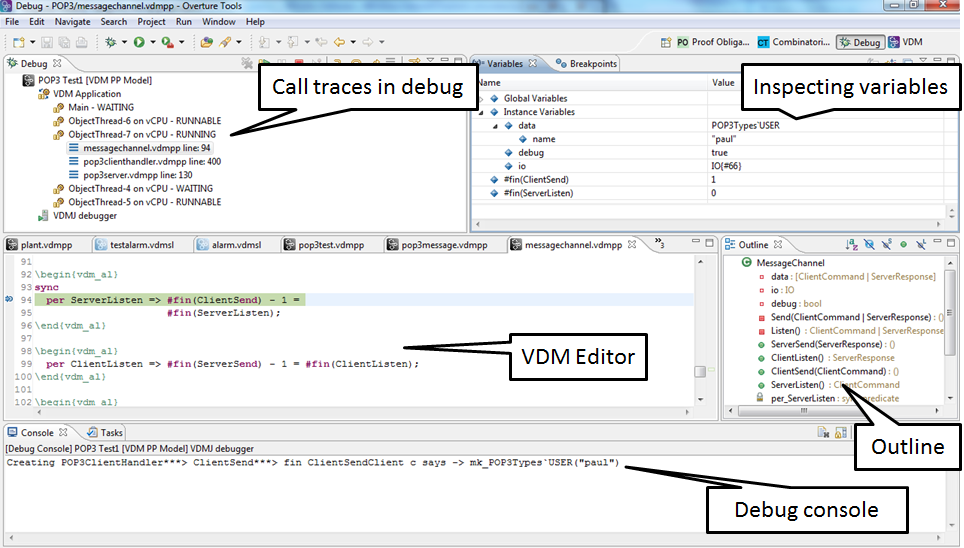
\includegraphics[width=5in]{figures/DebuggingVDM}
  \caption[Debugging perspective]{Debugging perspective}
  \label{fig:DebuggingVDM}
\end{center}
\end{figure}

The \emph{Debug view} in the upper left corner of the \emph{Debug
  perspective} shows all running threads in the VDM++ model and their
call stacks. It also shows whether a given model is stopped, suspended
or running. All threads are also shown, along with their running
status. It is possible to switch between threads from the \emph{Debug}
view\footnote{In the current version only the thread where the
  breakpoint is met is stopped, but in the future all threads will be
  stopped when a breakpoint is met and all will be enabled again once
  the user resume the execution.}.

\begin{table}
\begin{center}
\begin{tabular}{|l|l|}\hline \hline
\textbf{Button} & \textbf{Explanation} \\ \hline

\includegraphics[width=0.03\textwidth]{figures/resume} & Resume debugging \\

\includegraphics[width=0.03\textwidth]{figures/suspend} & Suspend debugging\\

\includegraphics[width=0.03\textwidth]{figures/terminate} & Terminate debugging\\

\includegraphics[width=0.03\textwidth]{figures/stepinto} & Step into\\

\includegraphics[width=0.03\textwidth]{figures/stepover} & Step over \\

\includegraphics[width=0.03\textwidth]{figures/stepreturn} & Step return\\

\includegraphics[width=0.03\textwidth]{figures/stepbystep} & Use step filters\\
\hline \hline
\end{tabular}
\caption{Overture debugging buttons\label{tab:debugButtons}}
\end{center}
\end{table}

At the top of the view are buttons for controlling debugging such as stop, step
into, step over and resume. These are standard Eclipse debugging
buttons~(see Table~\ref{tab:debugButtons}).

The \emph{Variables view} shows all the variables in a given context,
when a breakpoint is reached. The variables and their displayed values
are automatically updated when stepping through a model. The view is
located in the upper right corner in the Debug perspective.
%It is also possible to inspect complex
%variables, expanding nested arrays and so on.


\begin{figure}[htp]
\begin{center}
  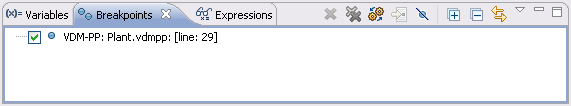
\includegraphics[width=4in]{figures/BreakpointView}
  \caption{Breakpoint View}
  \label{fig:BreakpointView}
\end{center}
\end{figure}

The \emph{Breakpoints view} gives an overview of all breakpoints set
(see Figure~\ref{fig:BreakpointView}). From this view you
can easily navigate to the location of a given breakpoint, disable or
delete them, or set their properties. 
%In figure
%\ref{fig:DebuggingVDM} the Breakpoints view is hidden behind the
%Variables view in the upper right hand corner in a tabbed notebook.
Conditional breakpoints are supported. These are a powerful tool for
the developer since they allow a condition to be specified which has
to be true in order for the debugger to stop at the given
breakpoint. The condition can either be a boolean expression using
variables in scope at the breakpoint, or it can be a hit count after
which the breakpoint should become active.

\begin{figure}[htp]
\begin{center}
  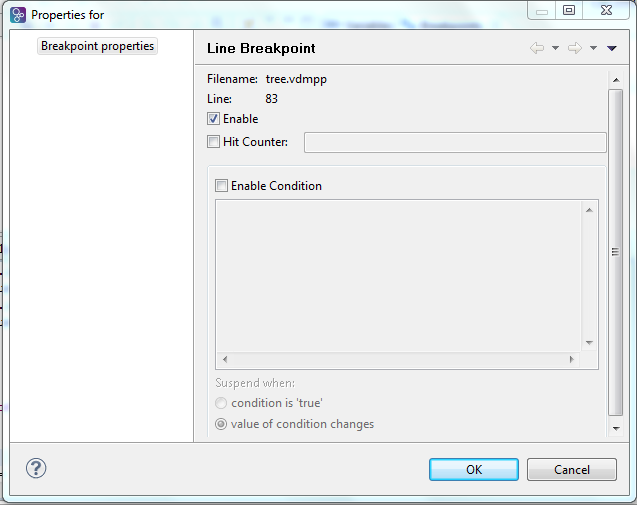
\includegraphics[width=4in]{figures/Breakpointconditional}
  \caption{Conditional breakpoint options}
  \label{fig:BreakpointConditional}
\end{center}
\end{figure}

You can make a simple breakpoint conditional by right clicking on the
breakpoint mark in the left margin of the editor and selecting the
option \emph{Breakpoint properties}. This opens a dialog shown in
Figure~\ref{fig:BreakpointConditional}.
%It is possible to choose
%between two different types of conditional: a hit count condition and one based
%on an expression defined by the user.

The \emph{Expressions view} allows the user to enter \emph{watch}
expressions whose values are automatically displayed and updated when
stepping. Watch expressions can be added manually or created by
selecting \emph{create watch expression} from the \emph{Variables} view. It
is possible to edit existing expressions.  Like the Breakpoints view,
this view is hidden in the upper right hand corner in
Figure~\ref{fig:DebuggingVDM}.

While the Overture Expressions view allows you to inspect values, the
functionality is somewhat limited. For more thorough inspections in
Overture, the \emph{Interactive Console view} is provided. Here
commands can be executed in a given context, i.e.\ when the debugger
is at a breakpoint. The Interactive Console keeps a command history,
so that previously executed commands can be run again easily. The
interactive console can be seen at the bottom of
Figure~\ref{fig:DebuggingVDM}.


\begin{myexercise}
\label{ex:tool-monitor}Use the interpreter to evaluate the
  following expression: {\ttfamily new Test1().Run()}.
\end{myexercise}

\section{Test coverage}\label{sec:testcov}

It is often useful to know how much of a model has been exercised by a
set of tests. This gives some insight into the thoroughness of a test
suite and may also help to identify parts of the model that have not
been assessed, allowing new tests to be devised to cover these. When
any evaluation is performed on a VDM++ model, the interpreter records
the lines of the VDM++ model that are executed. This permits the line
coverage to be examined after a test to identify the parts of the
VDM++ model that have not yet been exercised -- coverage is
cumulative, so a set of tests can be executed and their total coverage
examined at the end.

In our simple example, the different tests in the exercise above does
cause the majority of the VDM++ model to be executed, but for
demonstration purposes let us start by cleaning the model (right click
on the project and select \texttt{Clean}). If we simply take the
\texttt{AlarmErrPP} debug launch configuration the
\verb|ExpertIsOnDuty| function in \verb|plant.vdmpp| is called by the
\texttt{Run} function. Remember that whenever test coverage
information is desired the \texttt{Generate Latex Coverage} option
must be selected. Once the debugger has completed and the result
is written out in the \texttt{console} it is possible to right click
on the \texttt{AlarmErrPP} project and select the \emph{Latex} $
\rightarrow $ \emph{Latex coverage} the coverage information that have
been gathered in any expressions that have been debugged since the
last change to a file have been saved or the project have been cleaned
will be turned into a pdf file. The \texttt{AlarmErrPP.pdf} file is
placed in the \texttt{generated/latex} directory. Note that whenever the model is adjusted or it
is cleaned so it gets type checked again all the files in the
\texttt{generated} directory is deleted.

The coverage information is provided in a way where uncovered
expressions are shown in red in the generated pdf file. In addition
after the content of each VDM++ source file a table with coverage
overview is provided in tabular form. For the \texttt{plant.vdmpp}
file this looks like:

\begin{longtable}{|l|r|r|}
\hline
Function or operation & Coverage & Calls \\
\hline
\hline
ExpertIsOnDuty & 100.0\% & 1 \\
\hline
ExpertToPage & 100.0\% & 1 \\
\hline
NumberOfExperts & 0.0\% & 0 \\
\hline
Plant & 100.0\% & 1 \\
\hline
PlantInv & 100.0\% & 2 \\
\hline
\hline
plant.vdmpp & 89.0\% & 5 \\
\hline
\end{longtable}

\noindent where the \texttt{ExpertIsOnDuty} and \texttt{ExpertToPage} 
operations are fully covered
by just one call (due to the fact that its body is simply one line)
whereas the \texttt{PlantInv} operation is called 2 times.

\section{Combinatorial Testing}\label{sec:CT}

The previous sections have shown how to test and debug models
manually. However, Overture also contains a feature enabling more
automation in the testing process, making more comprehensive
high-volume testing feasible. It is possible to write regular
expressions, as \emph{traces}, that one would like to expand into a
large set of individual tests.

In order to illustrate how this can be used, we extend the
\texttt{Plant} class with two additional operations for adding and
removing experts from a given schedule. Both operations take a given
\texttt{Period} and an \texttt{Expert} and then update the
\texttt{schedule} instance variable from the \texttt{Plant} class. The
\texttt{AddExpertToSchedule} operation can be defined as:


\begin{lstlisting}
public AddExpertToSchedule: Period * Expert ==> ()
AddExpertToSchedule(p,ex) ==
  schedule(p) := if p in set dom schedule
                 then schedule(p) union {ex}
                 else {ex};
\end{lstlisting}

\noindent and the \texttt{RemoveExpertFromSchedule} operation can
be expressed as:

\begin{lstlisting}
public RemoveExpertFromSchedule: Period * Expert ==> ()
RemoveExpertFromSchedule(p,ex) == 
  let exs = schedule(p) in
    schedule := if card exs = 1
                then {p} <-: schedule
                else schedule ++ {p |-> exs \ {ex}}
pre p in set dom schedule;
\end{lstlisting}

\noindent Note that \texttt{RemoveExpertFromSchedule} contains a
deliberate error. It fails to take account of the invariant so the
operation can leave the \texttt{Plant} in a state where it cannot be
guaranteed that experts with the right qualifications are available in
the periods that have been scheduled. \texttt{AddExpertToSchedule} has
a similar error.  If nobody is scheduled at the period provided as an
argument, and the expert added for the schedule at this period does
not have all the necessary qualifications, the invariant will again be
violated. In fact this means that one would probably have to change
the signature of this operation such that it instead of taking a
simple expert would take a collection of experts.  We could use the
debugger presented above to test these two new operations manually,
but we can also automate a part of this process.

In order to do the automation, Overture needs to know about the
combinations of operation calls that you would like to have carried
out, so it is necessary to write a kind of regular expression called a
\emph{trace}. VDM++ has been extended such that traces can be written
directly as a part of a VDM++ model. A full explanation of this can be
found in~\cite{Larsen&09d}. In our case, inside the \texttt{Test2}
class one can write\footnote{Such \emph{traces} can actually also be
  represented as UML sequence diagrams and then automatically
  translated into the corresponding VDM++ textual form, but since this
is still at a prototyping stage it is not explained further here.}:

\begin{lstlisting}
traces

AddingAndDeleting: 
  let myex in set exs
  in
    let myex2 in set exs \ {myex}
    in
      let p in set ps 
      in
       (plant.AddExpertToSchedule(p,myex);
        plant.AddExpertToSchedule(p,myex2);
        plant.RemoveExpertFromSchedule(p,myex);
        plant.RemoveExpertFromSchedule(p,myex2));
\end{lstlisting}

\noindent The three nested let-be-such-that statements in the trace
called \texttt{AddingAndDeleting} yield all possible combinations of
their variable bindings whereas manual debugging will just select a
few combinations.  The cardinality of these sets determines the
overall number of test cases, each being formed as a sequence of four
operation calls, as shown. In this case, the cardinality of the three
sets are respectively 4, 3 and 4. Multiplying these gives 48. If you
select the Combinatorial Testing perspective you will see the
\textsf{CT Overview} view. Inside this view you can select the alarm
project, right click it and choose the \textsf{Run selected}
option. Now Overture expands and executes all 48 test cases one after
another. The results of these executions are illustrated with green
check marks and red crosses, meaning that the tests passed or failed
respectively. See Figure~\ref{fig:stracesalarm}. Note that in the
Combinatorial Testing perspective, the view in the lower region is
able to show the individual steps of a selected test case, along with
the corresponding results from its four operation calls.

\begin{figure}[htbp]
\begin{center}
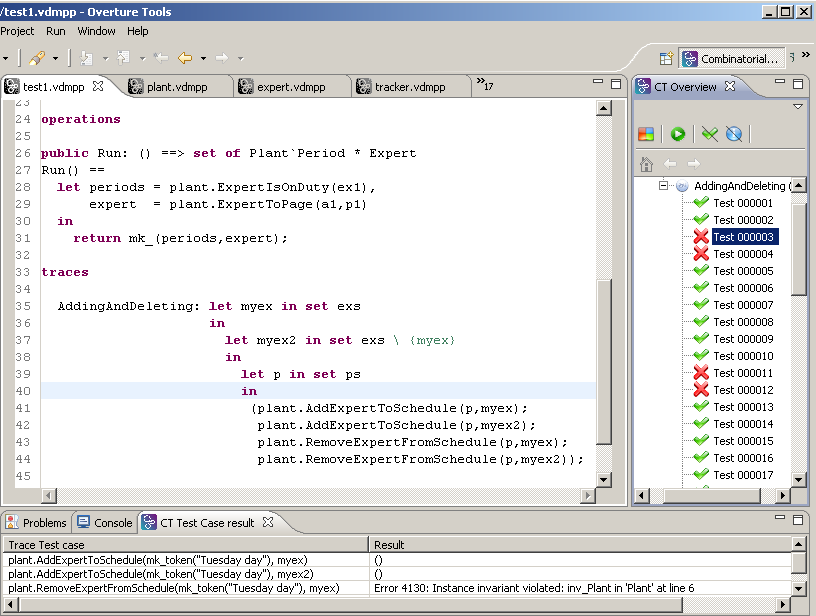
\includegraphics[width=4.5in]{figures/tracesalarm}
\caption{Using Combinatorial Testing for the Alarm VDM++ model\label{fig:stracesalarm}}
\end{center}
\end{figure}

The syntax for traces also enables operation repetition and alternatives to be
specified, but these were not needed for this simple case. Using the full power
of traces it is possible to efficiently generate and execute very large test
suites. Naturally, this is most likely to find inconsistencies when the model
attempts to define its essential predicates (invariants, pre and
post-conditions)\footnote{Note that when using repetitions and
  sequencing in combination it is easy to define traces that expands
  to hundreds of thousands of test cases and naturally their execution
  may then be very slow if one executes them all. Thus work is
  underway for a feature that reduce the numbers of tests to be
  executed using various intelligenet selection techniques. This will
  be released in a future version of Overture.}.

\section{Proof Obligations}\label{sec:PO}

The Overture tool is also able to generate \emph{Proof Obligations}
automatically for VDM++ models. Proof obligations are boolean
expressions that describe constraints to be met at various points in
the model in order to ensure that the model is internally consistent
(i.e.\ no run-time errors will occur while debugging if these are all
satisfied). Proof obligations are generated to ensure, for example,
that operations will always respect invariants on instance
variables. Each proof obligation generated from a model should
evaluate to \emph{true}.

The proof obligation generator is invoked by right clicking on the
project in the \emph{Explorer view} and then selecting the \emph{Proof
  Obligations} \texttt{->} \emph{Generate Proof Obligations}
entry. This will start up a proof obligation perspective with a
special \emph{PO view}. For the alarm example this view takes the form
shown in Figure~\ref{fig:POview}.

\begin{figure}[htbp]
\begin{center}
\includegraphics[width=4.5in]{figures/POview}
\caption{The Proof Obligation view for the Alarm VDM++ model\label{fig:POview}}
\end{center}
\end{figure}

One of the first proof obligations listed for this example is related
to the \texttt{PlantInv} function. Recall that the first part of the
function's definition is as follows:

\begin{lstlisting}
PlantInv: set of Alarm * map Period to set of Expert -> 
          bool
PlantInv(as,sch) ==
  (forall p in set dom sch & sch(p) <> {}) and ...
\end{lstlisting}

%Proof obligations can be produced either automatically from the command line
%with the \verb|-p| option, or they can be generated from the interactive prompt
%using the \verb|pog <function/operation>| command. In the case of our alarm
%example, most of the proof obligations concern the invariant on the Plant when
%changes of state occur, or the application of various map types, where the key
%being mapped must exist in the domain of the map. The \texttt{Test1} class itself also
%produces an obligation, meaning that we must verify that the two maplets in the
%Plant test data supplied are compatible:

The proof obligation records the constraint that the mapping application
\texttt{sch(p)} should be valid (i.e.\ that the \texttt{p} is in the
domain of the mapping \texttt{sch}). This is described as a proof
obligation in the following form:

\begin{lstlisting}
forall as:set of Alarm, sch:map Period to set of Expert &
  forall p in set (dom sch) &
    p in set dom sch
\end{lstlisting}
It is easy to see with simple pattern matching that this proof
obligation is true and thus in the \emph{Proof Obligation Explorer}
view the status field the small checkmark indicates that indeed the
proof obligation generation have been able to automatically determine
this. 

In general proof obligations represent checks that should be made on a
model in order to gain confidence in its consistency. At present,
proof obligations have to be checked by manual inspection of the model
code. Proof tools are being developed for Overture to check as many as
possible of the proof obligations automatically and with human
assistance, but there are always likely to be some that have to be
checked manually. If we for example instead consider the fifth proof
obligation it is derived from the body of the \texttt{expertToPage}
operation. That body looks like:

\begin{lstlisting}
  let expert in set schedule(p) be st
      a.GetReqQuali() in set expert.GetQuali()
  in
    return expert
\end{lstlisting}

\noindent where an expert on duty with the right qualifications are
being selected. The proof obligation here states:

\begin{lstlisting}
exists expert in set schedule(p) & 
   a.GetReqQuali() in set expert.GetQuali()
\end{lstlisting}

\noindent This is exactly describing that in order for this expression
to be defined it is necessary to gurantee that there exists at least
one such expert. Thus, without taking the pre-condition for the
operation here into account it would not be possible to gurantee
that. So it will never be possible to automatically to determin this
using simple pattern matching because this is only guranteed because
of the invariant over the instance variables for the \texttt{Plant}
class that has been defined.
 
\section{A Command-Line Interface}\label{sec:cmdline}

So far only the graphical user interface of Overture has been
presented but the engine underlying Overture, called VDMJ, also
provides a simple command line interface.  This is useful for the
automatic batch execution of tests, though the command line also
provides a full set of interactive execution and debugging commands
which can be useful when examining batch tests. The command line also
provides access to tool facilities that have not yet been included in
the Overture IDE.

VDMJ is written in Java, and so to run it from the command line, the
VDMJ jar file \footnote{See the Overture documentation at
  \texttt{sourceforge.net/projects/overture} for the location of the
  jar file.}  should be executed with a Java JRE (version 5 or later):

\lstset{style=tool,language=}
\begin{lstlisting}
java -jar vdmj-2.0.0.jar
\end{lstlisting}

\noindent If the jar file is executed with no further options like this, it will
print a list of available options and exit. The most important option is the VDM
dialect that the tool should use. In the case of our alarm example, we want to
use VDM++ for which the option is \verb|-vdmpp|. After this, we can simply
specify the names of the VDM model files to load, or the name of a
directory from which all VDM model files will be loaded:

\begin{lstlisting}
java -jar vdmj-2.0.0.jar -vdmpp AlarmPP
\end{lstlisting}

\noindent That will perform a syntax and type check of all the
VDM model files i the \verb|AlarmPP| directory, producing any
errors and warning messages on the console, before terminating:

\begin{lstlisting}
Parsed 4 classes in 0.561 secs. No syntax errors
Type checked 4 classes in 0.031 secs. No type errors
\end{lstlisting}

\noindent In the case of our alarm example, there are no syntax or
type checking errors. Any warnings can be suppressed using the
\verb|-w| option.

If a VDM model has no type checking errors, it can either be given
an expression to evaluate as an option on the command line, or the
user can enter an interactive mode to evaluate expressions and debug
their execution.

To evaluate an expression from the command line, the \verb|-e| option
is used, followed by a VDM expression to evaluate. You may also find
the \verb|-q| option useful, as this suppresses the informational
messages about the parsing and type checking:

\begin{lstlisting}
java -jar vdmj-2.0.0.jar -vdmpp -q -e "new Test1().Run()" 
AlarmPP
\end{lstlisting}

\noindent This produces a single line of output for the evaluation, since the
parsing and checking messages are suppressed:

\begin{lstlisting}
mk_({mk_token("Monday day")},
	Expert{#3, quali:={<Mech>, <Bio>}})
\end{lstlisting}

Clearly a batch of test evaluations could be performed automatically by running
a series of similar commands and saving the output results for comparison
against expected results.

To run the command line interpreter interactively, the \verb|-i| command line
option must be given. Instead of terminating after the type check, this will
cause VDMJ to enter its interactive mode, and give the interactive \verb|>|
prompt:

\begin{lstlisting}
Parsed 4 classes in 0.468 secs. No syntax errors
Type checked 4 classes in 0.031 secs. No type errors
Initialized 4 classes in 0.031 secs. 
Interpreter started
>  
\end{lstlisting}

\noindent From this prompt, various interactive commands can be given to
evaluate expressions, debug their evaluation, or examine the VDM model environment.
The \verb|help| command lists the commands available. The \verb|quit| command
leaves the interpreter.

For example, the following session illustrates the creation of a test object,
followed by an evaluation (using a \texttt{print} command)
of its \verb|Run| operation, and a debug
session with a breakpoint at the start of the same operation:

\begin{lstlisting}
> create test := new Test1()
> print test.Run()
= mk_({mk_token("Monday day")}, 
      Expert{#3, quali:={<Mech>, <Bio>}})
Executed in 0.172 secs.

> break Test1`Run
Created break [1] in 'Test1' (test1.vdmpp) at line 26:3
26:    let periods = plant.ExpertIsOnDuty(ex1),

> print test.Run()
Stopped break [1] in 'Test1' (test1.vdmpp) at line 26:3
26:    let periods = plant.ExpertIsOnDuty(ex1),
[thread 1]> print plant.NumberOfExperts(
                     mk_token("Wednesday"))
Runtime: Error 4071: Precondition failure: 
         pre_NumberOfExperts in 
         'Test1' (console) at line 1:1
[thread 1]> continue
= mk_({mk_token("Monday day")}, 
      Expert{#3, quali:={<Mech>, <Bio>}})
Executed in 91.014 secs. 
\end{lstlisting}

\noindent Notice that the \verb|print| command is available at the breakpoint
to examine the runtime state of the system. In the example, we attempt to evaluate an
operation which fails its precondition (because the system is not yet
initialized). The \verb|help| command is context sensitive, and will list the
extra debugging commands available at a breakpoint, such as \verb|continue|,
\verb|step|, \verb|stack|, \verb|list| and so on. The full set of commands is
described in the VDMJ User Guide\footnote{Supplied with the Overture
documentation.}.

\lstset{style=mystyle,language=VDM++}

\section{Summary}\label{sec:toolintrosummary}

In this guide we have introduced the following major features of tool
support for VDM++:
\begin{itemize}
\item using Enterprise Architect with class diagrams;
\item mapping back and forth between Enterprise Architect and Overture;
%\item configuration of selected VDM++ files;
\item syntax checking of VDM++ models;
\item type checking of VDM++ models;
%\item the notion of error messages;
\item executing and debugging VDM++ models;
\item collecting and displaying test coverage information on VDM++
  models;
%\item a command-line interface;
%\item pretty printing VDM++ models with test coverage information;
\item combinatorial testing enabling automation of parts of the
  testing process; 
\item proof obligation generation and
\item a command-line interface enabling access to test coverage.
%\item the existence of the application programming interface;
%\sindex{VDMTools@\vdmtools\ API}
%\item the existence of code generators; and
%\item setting tool and project options.\sindex{tool options@\tool{tool
%options}}\sindex{project options@\tool{project options}}
\end{itemize}


%\backmatter
\appendix

\bibliographystyle{newalpha}

\bibliography{book}

\appendix

\chapter{A Chemical Plant Example}\label{app:alarm}

This appendix presents the requirements for a simple alarm system for a
chemical plant. It forms a running example that serves to illustrate
the process described earlier and to introduce elements of the VDM++
modelling language. Although the modelling process is described here
as though it were a single-pass activity, a real development would
usually be iterative. 


\section{An informal description}



The example is inspired by a subcomponent of a large
alarm system developed by IFAD A/S and introduced in 
\cite{Fitzgerald&98b}. 
Chapter~\ref{cha:toolbox} provides an interactive and hands-on tour of
the tools available for supporting the development of the model.

Imagine that you are developing a system that manages the calling out
of experts to deal with operational faults discovered in a chemical
plant.  The plant is equipped with sensors that are able to raise
alarms in response to conditions in the plant.  When an alarm is
raised, an expert must be called to the scene.  Experts have different
qualifications for coping with different kinds of alarms. It has been
decided to produce a model to ensure that the rules
concerning the duty schedule and the calling out of experts are
correctly understood and implemented. The individual requirements are
labelled R1, R8 for further reference:

\begin{reqs}
\item A computer-based system is to be developed to manage the alarms 
of this plant.
\item Four kinds of qualifications are needed to cope with the alarms: 
 electrical, mechanical, biological, and chemical.
\item There must be experts on duty during all periods allocated in 
the system.
\item Each expert can have a list of qualifications.
\item Each alarm reported to the system has a qualification associated 
with it along with a description of the alarm that can be understood 
by the expert.
\item Whenever an alarm is received by the system an expert with the 
right qualification should be found so that he or she can be 
paged.
\item The experts should be able to use the system database to check 
when they will be on duty.
\item It must be possible to assess the number of experts on duty.
\end{reqs}

In the next section the development of a model of an alarm
system to meet these requirements is initiated. The purpose of the model is to
clarify the rules governing the duty roster and calling out of experts
to deal with alarms.

\section{A VDM-SL model of the Alarm example}\label{sec:VDMModel}

This section presents the full VDM-SL model
of the alarm example. However, it does so without any explanatory
text. That is placed in the VDM-SL book so if you are a newcommer to
VDM-SL please read that there.

\begin{lstlisting}
types

  Plant :: schedule : Schedule
           alarms   : set of Alarm
  inv mk_Plant(schedule,alarms) ==
        forall a in set alarms &
	   forall peri in set dom schedule &
	     QualificationOK(schedule(peri),a.quali);
	     
  Schedule = map Period to set of Expert
inv sch ==
   forall exs in set rng sch &
          exs <> {} and
          forall ex1, ex2 in set exs &
                 ex1 <> ex2 => ex1.expertid <> ex2.expertid;

  Period = token;

  Expert :: expertid : ExpertId
            quali    : set of Qualification
  inv ex == ex.quali <> {};

  ExpertId = token;

  Qualification = <Elec> | <Mech> | <Bio> | <Chem>;
	   
  Alarm :: alarmtext : seq of char
           quali     : Qualification
\end{lstlisting}

The functionality from the requirements presented above can be defined
in a number of functions as follows.

\begin{lstlisting}
functions

  NumberOfExperts: Period * Plant -> nat
  NumberOfExperts(peri,plant) ==
    card plant.schedule(peri)
  pre peri in set dom plant.schedule;

  ExpertIsOnDuty: Expert * Plant -> set of Period
  ExpertIsOnDuty(ex,mk_Plant(sch,-)) ==
    {peri| peri in set dom sch & ex in set sch(peri)};

  ExpertToPage(a:Alarm,peri:Period,plant:Plant) r: Expert
  pre peri in set dom plant.schedule and
      a in set plant.alarms
  post r in set plant.schedule(peri) and
       a.quali in set r.quali;

  QualificationOK: set of Expert * Qualification -> bool
  QualificationOK(exs,reqquali) ==
    exists ex in set exs & reqquali in set ex.quali
\end{lstlisting}

The \texttt{ChangeExpert} function below is not correct but it is used
for exercise/test purposes in this tutorial.

\begin{lstlisting}
functions

ChangeExpert: Plant * Expert * Expert * Period -> Plant
ChangeExpert(mk_Plant(plan,alarms),ex1,ex2,peri) ==
  mk_Plant(plan ++ {peri |-> plan(peri)\{ex1} union {ex2}},
           alarms)
\end{lstlisting}

In order to test the model different values can be defined. Such value
definitions make use of the types defined in the VDM-SL model.

\begin{lstlisting}
values
 
  p1:Period = mk_token("Monday day");
  p2:Period = mk_token("Monday night");
  p3:Period = mk_token("Tuesday day");
  p4:Period = mk_token("Tuesday night");
  p5:Period = mk_token("Wednesday day");
  ps : set of Period = {p1,p2,p3,p4,p5};

  eid1:ExpertId = mk_token(134);
  eid2:ExpertId = mk_token(145);
  eid3:ExpertId = mk_token(154);
  eid4:ExpertId = mk_token(165);
  eid5:ExpertId = mk_token(169);
  eid6:ExpertId = mk_token(174);
  eid7:ExpertId = mk_token(181);
  eid8:ExpertId = mk_token(190);
  
  e1:Expert = mk_Expert(eid1,{<Elec>});
  e2:Expert = mk_Expert(eid2,{<Mech>,<Chem>});
  e3:Expert = mk_Expert(eid3,{<Bio>,<Chem>,<Elec>});
  e4:Expert = mk_Expert(eid4,{<Bio>});
  e5:Expert = mk_Expert(eid5,{<Chem>,<Bio>});
  e6:Expert = mk_Expert(eid6,{<Elec>,<Chem>,<Bio>,<Mech>});
  e7:Expert = mk_Expert(eid7,{<Elec>,<Mech>});
  e8:Expert = mk_Expert(eid8,{<Mech>,<Bio>});
  exs : set of Expert = {e1,e2,e3,e4,e5,e6,e7,e8};

  s: map Period to set of Expert
     = {p1 |-> {e7,e5,e1},
        p2 |-> {e6},
        p3 |-> {e1,e3,e8},
        p4 |-> {e6}};

  a1:Alarm = mk_Alarm("Power supply missing",<Elec>);
  a2:Alarm = mk_Alarm("Tank overflow",<Mech>);
  a3:Alarm = mk_Alarm("CO2 detected",<Chem>);
  a4:Alarm = mk_Alarm("Biological attack",<Bio>);
  alarms: set of Alarm = {a1,a2,a3,a4};

  plant1: Plant = mk_Plant(s,{a1,a2,a3,a4})
\end{lstlisting}  

A basic explicit operation for test purposes can be defined as below.

\begin{lstlisting}  
operations

Run: Expert ==> set of Period
Run(e) == return ExpertIsOnDuty(e, plant1);
\end{lstlisting}

In the new VDM-10 variant of VDM-SL {\bf\ttfamily traces} have been
incorporated since they can be used with tool support for
combinatorial testing purposes.

\begin{lstlisting}
traces

  Test1: let a in set alarms
         in
           let p in set ps 
           in
             (NumberOfExperts(p,plant1);
              pre_ExpertToPage(a,p,plant1);
              let ex in set exs
              in
                post_ExpertToPage(a,p,plant1,ex))
               
  Test2: let ex in set exs
         in
           ExpertIsOnDuty(ex,plant1)
\end{lstlisting}  


\end{document}
